\chapter{Mengenal Kecerdasan Buatan dan Scikit-Learn}
Buku umum yang digunakan adalah \cite{russell2016artificial} dan  
untuk sebelum UTS menggunakan buku \textit{Python Artificial Intelligence Projects for Beginners}\cite{eckroth2018python}.
Dengan praktek menggunakan python 3 dan editor anaconda dan library python scikit-learn.
Tujuan pembelajaran pada pertemuan pertama antara lain:
\begin{enumerate}
\item
Mengerti definisi kecerdasan buatan, sejarah kecerdasan buatan, perkembangan dan penggunaan di perusahaan
\item
Memahami cara instalasi dan pemakaian sci-kit learn
\item
Memahami cara penggunaan variabel explorer di spyder
\end{enumerate}
Tugas dengan cara dikumpulkan dengan pull request ke github dengan menggunakan latex pada repo yang dibuat oleh asisten riset.

\section{Teori}
Praktek teori penunjang yang dikerjakan :
\begin{enumerate}
\item
Buat Resume Definisi, Sejarah dan perkembangan Kecerdasan Buatan, dengan bahasa yang mudah dipahami dan dimengerti. Buatan sendiri bebas plagiat[hari ke 1](10)
\item
Buat Resume mengenai definisi supervised learning, klasifikasi, regresi dan unsupervised learning. Data set, training set dan testing set.[hari ke 1](10)
\end{enumerate}

\section{Instalasi}
Membuka https://scikit-learn.org/stable/tutorial/basic/tutorial.html. Dengan menggunakan bahasa yang mudah dimengerti dan bebas plagiat. 
Dan wajib skrinsut dari komputer sendiri.
\begin{enumerate}
\item
Instalasi library scikit dari anaconda, mencoba kompilasi dan uji coba ambil contoh kode dan lihat variabel explorer[hari ke 1](10)
\item
Mencoba Loading an example dataset, menjelaskan maksud dari tulisan tersebut dan mengartikan per baris[hari ke 1](10)
\item
Mencoba Learning and predicting, menjelaskan maksud dari tulisan tersebut dan mengartikan per baris[hari ke 2](10)
\item
mencoba Model persistence, menjelaskan maksud dari tulisan tersebut dan mengartikan per baris[hari ke 2](10)
\item 
Mencoba Conventions, menjelaskan maksud dari tulisan tersebut dan mengartikan per baris[hari ke 2](10)
\end{enumerate}


\section{Penanganan Error}
Dari percobaan yang dilakukan di atas, apabila mendapatkan error maka:

\begin{enumerate}
	\item
	skrinsut error[hari ke 2](10)
	\item
Tuliskan kode eror dan jenis errornya [hari ke 2](10)
	\item
Solusi pemecahan masalah error tersebut[hari ke 2](10)

\end{enumerate}


\section{andi muh aslam/1164064}
\subsection{sejarah dan perkembangan kecerdasan buatan}
\begin{enumerate}
\item didefinisikan  kecerdasan yang ditunjukkan oleh suatu entitas buatan. Umumnya dianggap komputer. Kecerdasan Buatan (Artificial Intelligence atau AI) didefinisikan sebagai kecerdasan yang ditunjukan oleh suatu entitas buatan. Sistem seperti ini umumnnya dianggao kemputer. Kecerdasan dimasukkan ke dalam mesin (komputer) agar dapat melakukan pekerjaan seperti yang dapat dilakukan manusia. Kecerdasan Buatan (Artificial Intelligence atau AI) didefinikasikan sebagai kecerdasan yang ditinjukkan oleh suatu entitas buatan. Sistem seperti ini umumnya di anggap komputer. Kecerdasan diciptakan dan dimasukkan melakukan pekerjaan seperti yang dapat dilakukan manusia. 
\item Sejarah dan perkembangan kecerdasan buatan terjadi pada musim panas tahun 1956 tercatat adanya seminar mengenai AI di Darmouth College. Seminar pada waktu itu dihadiri oleh sejumlah pakar komputer dan membahas potensi komputer dalam meniru 
kepandaian manusia. Akan tetapi perkembangan yang sering terjadi semenjak diciptakannya LISP, yaitu bahasa kecerdasan buatan yang dibuat tahun 1960 oleh John McCarthy. Istilah pada kecerdasan buatan atau Artificial Intelligence diambil dari Marvin Minsky dari MIT. Dia menulis karya ilmiah berjudul Step towards Artificial Intelligence,The Institute of radio Engineers Proceedings 49, January 1961\cite{nasution2012implementasi}.
\item Supervised learning merupakan sebuah pendekatan dimana sudah terdapat data yang dilatih, dan terdapat variable yang ditargetkan sehingga tujuan dari pendekatan ini adalah mengkelompokan suatu data ke data yang sudah ada. Sedangkan unsupervised 
learning tidak memiliki data latih, sehingga dari data yang ada, kita mengelompokan data tersebut menjadi 2 bagian atau 3 bagian dan seterusnya.
\item Klasifikasi adalah salah satu topik utama dalam data mining atau machine learning. Klasifikasi yaitu suatu pengelompokan data dimana data yang digunakan tersebut mempunyai kelas label atau target.
\item Regresi adalah Supervised learning tidak hanya mempelajari classifier, tetapi juga mempelajari fungsi yang dapat memprediksi suatu nilai numerik. Contoh, ketika diberi foto seseorang, kita ingin memprediksi umur, tinggi, dan berat orang yang ada pada foto tersebut.
\item Data set adalah cabang aplikasi dari Artificial Intelligence/Kecerdasan Buatan yang fokus pada pengembangan sebuah sistem yang mampu belajar sendiri tanpa harus berulang kali di program oleh manusia.
\item Training set yaitu jika pasangan objek, dan kelas yang menunjuk pada objek tersebut adalah suatu contoh yang telah diberi label akan menghasilkan suatu algoritma pembelajaran.
\subitem Testing set digunakan untuk mengukur sejauh mana classifier berhasil melakukan klasifikasi dengan benar\cite{darujati2012pemanfaatan}.
\end{enumerate}


\section{Instalasi}
\subsection{instalasi Library Scikit dari Anaconda}
\begin{enumerate}
\item Download aplikasi Anaconda terlebih dahulu
\begin{figure} [ht]
\centering
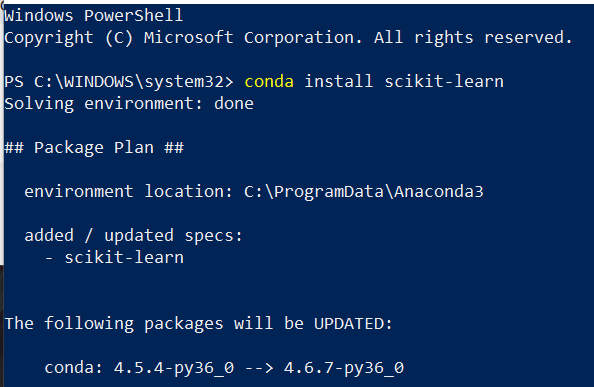
\includegraphics[scale=1] {figures/1.png}
\caption{Langkah 1 instalasi anaconda..}
\end{figure}

\item Proceed install anaconda 
\begin{figure} [ht]
\centering
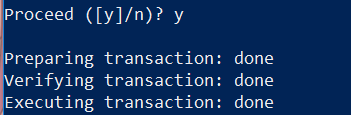
\includegraphics[scale=1] {figures/2.png}
\caption{Langkah 2 instalasi anaconda.}
\end{figure}

\item install scikit-learn
\begin{figure} [ht]
\centering 
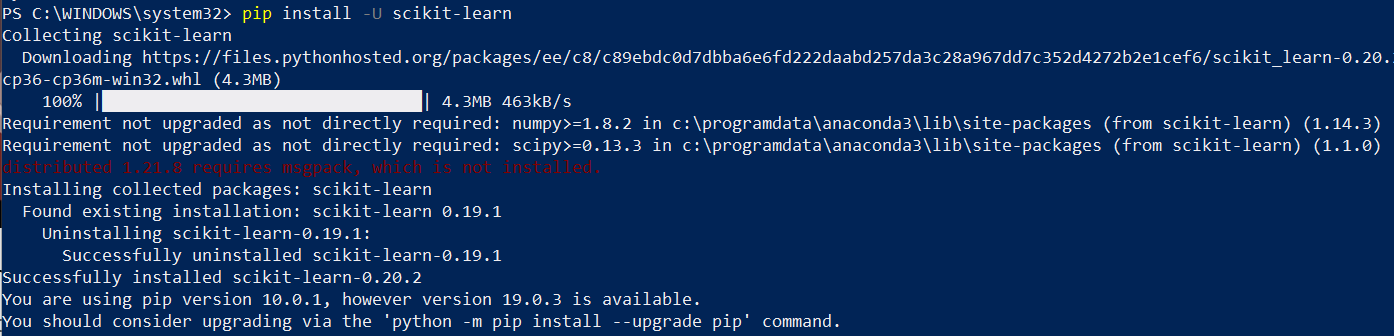
\includegraphics[scale=1] {figures/4.png}
\caption{Langkah 3 instalasi anaconda. }
\end{figure}

\item perintah print
\begin{figure} [ht]
\centering 
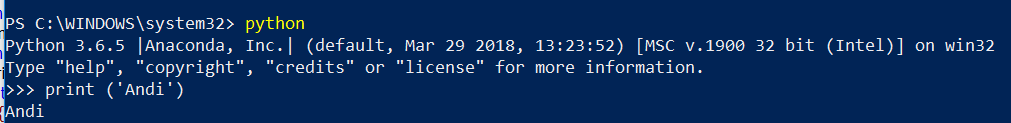
\includegraphics[scale=1] {figures/5.png}
\caption{Langkah 4 instalasi anaconda. }
\end{figure}
\end{enumerate}

\subsubsection{Mencoba Loading an example dataset}
\begin{enumerate}
\item Masuk Pyhton terlebih dahulu
\begin{figure} [ht]
\centering 
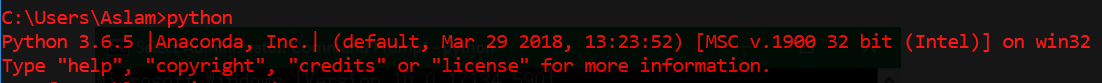
\includegraphics[scale=1] {figures/6.png}
\caption{Langkah 1 dataset. }
\end{figure}

\item from sklearn import datasets(pada baris ini merupakan sebuah perintah untuk mengimport sebuah datasets dari file sklearn).
\begin{figure} [ht]
\centering 

\includegraphics[scale=1] {figures/7.png}
\caption{Langkah 2 dataset. }
\end{figure}

\item iris \= datasets.load\_iris()(pada baris kedua ini dimana iris merupakan suatu variable yang berfungsi untuk mengambil data pada datasets dengan perintah .load\_iris).
\begin{figure} [ht]
\centering 

\includegraphics[scale=1] {figures/8.png}
\caption{Langkah 3 dataset. }
\end{figure}

\item digits \= datasets.load\_digits()(pada baris ketiga ini dimana digits merupakan suatu variable yang berfungsi untuk mengambil data pada datasets dengan perintah .load\_digits)
\begin{figure} [ht]
\centering 

\includegraphics[scale=1] {figures/9.png}
\caption{Langkah 4 dataset. }
\end{figure}

\item print(digits.data)(pada baris keempat ini merupakan perintah yang berfungsi untuk memanggil atau menampilkan variable digits.data)
\begin{figure} [ht]
\centering 
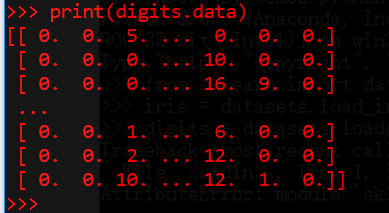
\includegraphics[scale=1] {figures/10.png}
\caption{Langkah 5 dataset. }
\end{figure}
\end{enumerate}

\subsubsection{Learning and Predicting}
\begin{itemize}
\item from sklearn import svm(pada baris ini merupakan sebuah perintah untuk mengimport class svm dari packaged sklearn).
\item clf = svm.SVC(gamma=0.001, C=100.)(pada baris kedua ini clf sebagai estimator/parameter, svm.SVC sebagai class, gamma sebagai parameter untuk menetapkan nilai secara manual)
\item clf.fit(digits.data[:-1], digits.target[:-1])(pada baris ketiga ini clf sebagai estimator/parameter, fit sebagai metode, digits.data sebagai item, [:-1] sebagai syntax pythonnya dan menampilkan outputannya) Lihat gambar 1.13.
\item clf.predict(digits.data[-1:])
\end{itemize}

\subsubsection{Model Presistence}
\begin{itemize}
\item from sklearn import svm(pada baris ini merupakan sebuah perintah untuk mengimport class svm dari packaged sklearn).
\item from sklearn import datasets(pada baris ini merupakan sebuah perintah untuk mengimport class datasets dari packaged sklearn).
\item\begin{verbatim} clf = svm.SVC(gamma='scale')\end{verbatim}(pada baris ketga ini clf sebagai estimator/parameter, svm.SVC sebagai class, gamma sebagai parameter untuk menetapkan nilai secara manual dengan nilai scale).
\item\begin{verbatim} iris = datasets.load_iris()\end{verbatim}(pada baris keempat ini iris sebagai estimator/parameter, datasets.load\_iris() sebagai item dari suatu nilai).
\item\begin{verbatim} X, y = iris.data, iris.target\end{verbatim}(pada baris kelima ini X, y sebagai estimator/parameter, iris.data, iris.target sebagai item dari 2 nilai yang ada).
\item\begin{verbatim} clf.fit(X, y)\end{verbatim}(pada baris keenam ini clf sebagai estimator/parameter dengan menggunakan metode fit untuk memanggil estimator X, y dengan outputannya) 
\item\begin{verbatim} import pickle\end{verbatim}(pickle merupakaan sebuah class yang di import).
\item\begin{verbatim} s = pickle.dumps(clf)\end{verbatim}(pada baris ini s sebagai estimator/parameter dengan pickle.dumps merupakan suatu nilai/item dari estimator/parameter clf)
\item\begin{verbatim} clf2 = pickle.loads(s)\end{verbatim}(pada baris ini clf2 sebagai estimator/parameter, pickle.loads sebagai suatu item, dan s sebagai estimator/parameter yang dipanggil) 
\item\begin{verbatim} clf2.predict(X[0:1])\end{verbatim}(pada baris ini clf2.predict sebagai suatu item dengan menggunakan metode predict untuk menentukkan suatu nilai dari (X[0:1])) 
\item\begin{verbatim} y[0]\end{verbatim}(pada estimator/parameter y berapapun angka yang diganti nilainya akan selalu konstan yaitu 0)
\item\begin{verbatim} from joblib import dump, load\end{verbatim}(pada baris berikut ini merupakan sebuah perintah untuk mengimport class dump, load dari packaged joblib).
\item\begin{verbatim} dump(clf, 'filename.joblib')\end{verbatim}(pada baris berikutnya dump di sini sebagai class yang didalamnya terdapat nilai dari suatu item clf dan data joblib).
\item\begin{verbatim} clf = load('filename.joblib')\end{verbatim}(pada baris terakhir clf sebagai estimato/parameter dengan suatu nilai load berfungsi untuk mengulang data sebelumnya)
\item dari ketiga baris akhir tersebut jika di jalankan aau dituliskan perintah seperti itu maka akan menampilkan tampilan eror 
\end{itemize}

\subsubsection{Conventions}
\begin{enumerate}
\item Type Casting
\begin{itemize}
\item\begin{verbatim} from sklearn import svm\end{verbatim}(pada baris ini merupakan sebuah perintah untuk mengimport class svm dari packaged sklearn).
\item\begin{verbatim} from sklearn import random_projection\end{verbatim}(pada baris ini merupakan sebuah perintah untuk mengimport class random\_projection dari packaged sklearn).
\item\begin{verbatim} rng = np.random.RandomState(0)\end{verbatim}(rng sebagai estimator/parameter dengan nilai suatu itemnya yaitu np.random.RandomState(0)).
\item\begin{verbatim} X = rng.rand(10, 2000)\end{verbatim}(X sebagai estimator/parameter dengan nilai item rng.rand).
\item\begin{verbatim} X = np.array(X, dtype='float32')\end{verbatim}(X sebagai estimator/parameter dengan nilai item np.array).
\item\begin{verbatim} X.dtype\end{verbatim}(X.dtype sebagai item pemanggil) 
\item\begin{verbatim} transformer = random_projection.GaussianRandomProjection()\end{verbatim}(transformer sebagai estimator/parameter dengan memanggil class random\_projection).
\item\begin{verbatim} X_new = transformer.fit_transform(X)\end{verbatim}(X\_new di sini sebagai estomator/parameter dan menggunakan metode fit)
\item\begin{verbatim} X_new.dtype\end{verbatim}(X\_new.dtype sebagai item) 
\item\begin{verbatim} from sklearn import datasets\end{verbatim}(pada baris ini merupakan sebuah perintah untuk mengimport class datasets dari packaged sklearn).
\item\begin{verbatim} from sklearn.svm import SVC\end{verbatim}(pada baris ini merupakan sebuah perintah untuk mengimport class SVC dari packaged sklearn.svm).
\item\begin{verbatim} iris = datasets.load_iris()\end{verbatim}(iris sebagai estimator/parameter dengan item datasets.load\_iris()).
\item\begin{verbatim} clf = SVC(gamma='scale')\end{verbatim}(clf sebagai estimator/parameter dengan nilai class SVC pada parameter gamma sebagai set penilaian).
\item\begin{verbatim} clf.fit(iris.data, iris.target)\end{verbatim}(estimator/parameter clf menggunakan metode fit dengan itemnya) 
\item\begin{verbatim} list(clf.predict(iris.data[:3]))\end{verbatim}(menambahkan item list dengan metode predict) 
\item\begin{verbatim} clf.fit(iris.data, iris.target_names[iris.target])\end{verbatim}(estimator/parameter clf menggunakan metode fit dengan itemnya)
\item\begin{verbatim} list(clf.predict(iris.data[:3]))(menambahkan item list dengan metode predict\end{verbatim} 
\end{itemize}
\item Refitting and Updating Parameters
\begin{itemize}
\item\begin{verbatim} import numpy as np\end{verbatim}(pada baris ini merupakan sebuah perintah untuk mengimport class svm dari np).
\item\begin{verbatim} from sklearn.svm import SVC\end{verbatim}(pada baris ini merupakan sebuah perintah untuk mengimport class SVC dari packaged sklearn.svm).
\item\begin{verbatim} rng = np.random.RandomState(0)\end{verbatim}(rng sebagai estimator/parameter dengan nilai suatu itemnya yaitu np.random.RandomState(0)).
\item\begin{verbatim} X = rng.rand(100, 10)\end{verbatim}(X sebagai estimator/parameter dengan nilai item rng.rand).
\item\begin{verbatim} y = rng.binomial(1, 0.5, 100)\end{verbatim}(y sebagai estimator/parameter dengan nilai item rng.binomial).
\item\begin{verbatim} X_test = rng.rand(5, 10)\end{verbatim}(X\_test sebagai estimator/parameter dengan nilai item rng.rand).
\item\begin{verbatim} clf = SVC()\end{verbatim}(clf sebagai estimator/parameter dan class SVC)
\item\begin{verbatim} clf.set_params(kernel='linear').fit(X, y)\end{verbatim}(set\_params sebagai item)
\item\begin{verbatim} clf.predict(X_test)\end{verbatim}(menggunakan metode predict) 
\item\begin{verbatim} clf.set_params(kernel='rbf', gamma='scale').fit(X, y)\end{verbatim} 
\item\begin{verbatim} clf.predict(X_test)\end{verbatim}
\end{itemize}
\item Multiclass vs. Multilabel Fitting
\begin{itemize}
\item\begin{verbatim} from sklearn.svm import SVC\end{verbatim}(pada baris ini merupakan sebuah perintah untuk mengimport class SVC dari packaged sklearn.svm).
\item\begin{verbatim} from sklearn.multiclass import OneVsRestClassifier\end{verbatim}(pada baris ini merupakan sebuah perintah untuk mengimport class OneVsRestClassifier dari packaged sklearn.multiclass).
\item\begin{verbatim} from sklearn.preprocessing import LabelBinarizer\end{verbatim}(pada baris ini merupakan sebuah perintah untuk mengimport class LabelBinarizer dari packaged sklearn.preprocessing).
\item\begin{verbatim} X = [[1, 2], [2, 4], [4, 5], [3, 2], [3, 1]]\end{verbatim}
\item\begin{verbatim} y = [0, 0, 1, 1, 2]\end{verbatim}
\item\begin{verbatim} classif = OneVsRestClassifier(estimator=SVC(gamma='scale',random_state=0))\end{verbatim}
\item\begin{verbatim} classif.fit(X, y).predict(X)\end{verbatim}
\item\begin{verbatim} y = LabelBinarizer().fit_transform(y)\end{verbatim}
\item\begin{verbatim} classif.fit(X, y).predict(X)\end{verbatim} 
\item\begin{verbatim} from sklearn.preprocessing import MultiLabelBinarizer\end{verbatim}
\item\begin{verbatim} y = [[0, 1], [0, 2], [1, 3], [0, 2, 3], [2, 4]]\end{verbatim}
\item\begin{verbatim} y = MultiLabelBinarizer().fit_transform(y)\end{verbatim}
\item\begin{verbatim} classif.fit(X, y).predict(X)\end{verbatim} 
\end{itemize}
\end{enumerate}

\subsection{Penanganan eror}
\subsubsection{ScreenShoot Eror}
\begin{figure}[ht]\centerline{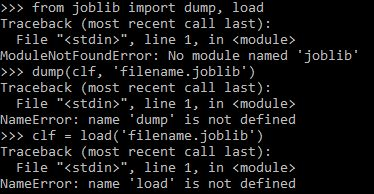
\includegraphics[width=0.75\textwidth]{figures/18.JPG}}\caption{Hasil Tampilan Error.}\end{figure}
\subsubsection{Tuliskan Kode Eror dan Jenis Erornya}
\begin{itemize}
\item \begin{verbatim}from joblib import dump, load\end{verbatim} (Kode baris pertama)
\subitem \begin{verbatim}
Traceback(most recent call last):
 File "<stdin>", line 1, in<module>
ModuleNotFoundError: No module named 'joblib'
\end{verbatim} (Errornya)
\item \begin{verbatim}dump(clf, 'filename.joblib')\end{verbatim} (Kode baris kedua)
\subitem \begin{verbatim}
Traceback(most recent call last):
 File "<stdin>", line 1, in<module>
NameError: name 'dump' is not defined
\end{verbatim} (Errornya)
\item \begin{verbatim}clf = load('filename.joblib')\end{verbatim} (Kode baris ketiga)
\subitem \begin{verbatim}
Traceback(most recent call last):
 File "<stdin>", line 1, in<module>
NameError: name 'load' is not defined
\end{verbatim} (Errornya)
\end{itemize}

\subsubsection{Solusi Pemecahan Masalah Error}
\begin{enumerate}
\item Pada masalah error sebelumnya itu dikarenakan kita belum mempunyai packaged joblib. Jadi solusinya yaitu dengan cara menginstall terlebih dahulu packaged joblibnya setelah itu baru perintah tersebut dapat dijalankan

\begin{figure}[ht]\centerline{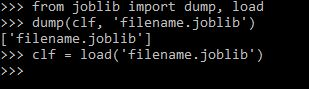
\includegraphics[width=0.75\textwidth]{figures/32.JPG}}\caption{Hasil Tampilan Uji coba perintah joblib.}\end{figure}
\end{enumerate}




